\documentclass[PermutationsCombinationsWhyWholeNumber.tex]{subfiles}
\title{Appendix: Why a combination, $\Combination{n}{k}$, is always a natural number? Different way to look at the answer accentuates the generation process of factors and prime numbers contained within a particular range of $1$ to $n$.}
\author{Amit Kumar}
\date{}
\usepackage[a4paper, margin=0.75in]{geometry}
\usepackage[page]{appendix}
\usepackage{amsmath}
\usepackage{amssymb}
\usepackage{mathtools}
\usepackage{xcolor}
\usepackage{ulem}
\usepackage{cancel}
\usepackage{listings}
\usepackage{pythonhighlight}
\usepackage{graphicx}
\usepackage{float}
\usepackage{url}
\usepackage{subfiles}
\usepackage{xr}
\externaldocument{PermutationsCombinationsWhyWholeNumber}
\begin{document}
	\maketitle
\begin{appendices}
	\section{Code to generate the plots as in \ref{Summary}}\label{PythonCodeToGenerateGraph}
	\begin{python}
#!/use/bin/python
"""
This module visualizes the graphs for a particular combination nCk.
create_chart_combination functions creates all x and y so that it can be plotted.
There are two functions:
(1) create_all_cases_graph: for all k(s) for a given n
(2) create_one_case_graph: for a specific k for a given n
There are 6 helper function depending n is even and if k has l or m.
All the files are saved to the current directory.
"""
from math import ceil, sqrt
from typing import Union
import matplotlib.pyplot as plt
from matplotlib.ticker import MaxNLocator

## Constants. Please do not change
GRAPH_TITLE = '$ ^{%d}C_{%d}$'
TEXTCOORDS = 'offset pixels'
##################################

def helper_even_not_l_m(each_x:int,
                        n:int,
                        k:int,
                        a:list[int],
                        y: list[int],
                        indiv_solution_params:list[tuple[Union[int,bool], Union[int,bool], Union[int,bool]]],
                        starting_guess:int=1,
                        l:bool=False,
                        not_l_m:bool=True,
                        m:bool=False)->None:
    """
    This function prepares y and individual params if n is even and both l amd m are zero for k.
    """
    while True:
        y_ = (starting_guess-1)*\floordivision{n}{2} - (starting_guess*each_x)
        if y_ > (2*(\floordivision{n}{2})-k):
            break                    
        if y_ >= 1:
            a.append(starting_guess)
            indiv_solution_params.append((l,not_l_m,m,starting_guess))
        starting_guess += 1
    y_s = list(map(lambda a_dash: (a_dash-1)*\floordivision{n}{2} - (a_dash*each_x),a))
    y.append(y_s)

def helper_even_l(each_x:int,
                        n:int,
                        k:int,
                        a:list[int],
                        y: list[int],
                        indiv_solution_params:list[tuple[Union[int,bool], Union[int,bool], Union[int,bool]]],
                        starting_guess:int=1,
                        l:bool=True,
                        not_l_m:bool=False,
                        m:bool=False)->None:
    """
    This function prepares y and individual params if n is even and m is zero for k but not l.
    """    
    while True:
        y_ = (starting_guess-1)*(\floordivision{n}{2}) + l*(starting_guess+1) - (starting_guess*each_x)
        if y_ > (2*(\floordivision{n}{2})-k):
            break
        if y_ >= 1:
            a.append(starting_guess)
            indiv_solution_params.append((l,not_l_m,m,starting_guess))
        starting_guess += 1
    y_s = list(map(lambda a_dash: (a_dash-1)*(\floordivision{n}{2}) +l*(a_dash+1) - (a_dash*each_x),a))
    y.append(y_s)    

def helper_even_m(each_x:int,
                        n:int,
                        k:int,
                        a:list[int],
                        y: list[int],
                        indiv_solution_params:list[tuple[Union[int,bool], Union[int,bool], Union[int,bool]]],
                        starting_guess:int=1,
                        l:bool=False,
                        not_l_m:bool=False,
                        m:bool=True)->None:
    """
    This function prepares y and individual params if n is even and l is zero for k but not m.
    """   
    while True:
        y_ = (starting_guess-1)*(\floordivision{n}{2}) -m*(starting_guess+1) - (starting_guess*each_x)
        if y_ > (2*(\floordivision{n}{2})-k):
            break                    
        if y_ >= 1:
            a.append(starting_guess)
            indiv_solution_params.append((l,not_l_m,m,starting_guess))
        starting_guess += 1
    y_s = list(map(lambda a_dash: (a_dash-1)*(\floordivision{n}{2}) -m*(a_dash+1) - (a_dash*each_x),a))
    y.append(y_s)    

def helper_noteven_not_l_m(each_x:int,
                        n:int,
                        k:int,
                        a:list[int],
                        y: list[int],
                        indiv_solution_params:list[tuple[Union[int,bool], Union[int,bool], Union[int,bool]]],
                        starting_guess:int=1,
                        l:bool=False,
                        not_l_m:bool=True,
                        m:bool=False)->None:
    """
    This function prepares y and individual params if n is odd and both l amd m are zero for k.
    """    
    while True:
        y_ = (starting_guess-1)*(\floordivision{n}{2}) +starting_guess - (starting_guess*each_x)
        if y_ > ((2*(\floordivision{n}{2})+1)-k):
            break                    
        if y_ >= 1:
            a.append(starting_guess)
            indiv_solution_params.append((l,not_l_m,m,starting_guess))
        starting_guess += 1
    y_s = list(map(lambda a_dash: (a_dash-1)*(\floordivision{n}{2})+a_dash - (a_dash*each_x),a))
    y.append(y_s)

def helper_noteven_l(each_x:int,
                        n:int,
                        k:int,
                        a:list[int],
                        y: list[int],
                        indiv_solution_params:list[tuple[Union[int,bool], Union[int,bool], Union[int,bool]]],
                        starting_guess:int=1,
                        l:bool=True,
                        not_l_m:bool=False,
                        m:bool=False)->None:
    """
    This function prepares y and individual params if n is odd and m is zero for k but not l.
    """   
    while True:
        y_ = (starting_guess-1)*(\floordivision{n}{2}) +starting_guess + l*(starting_guess+1) - (starting_guess*each_x)
        if y_ > ((2*(\floordivision{n}{2})+1)-k):
            break                    
        if y_ >= 1:
            a.append(starting_guess)
            indiv_solution_params.append((l,not_l_m,m,starting_guess))
        starting_guess += 1
    y_s = list(map(lambda a_dash: (a_dash-1)*(\floordivision{n}{2})+a_dash +l*(a_dash+1) - (a_dash*each_x),a))
    y.append(y_s)    

def helper_noteven_m(each_x:int,
                        n:int,
                        k:int,
                        a:list[int],
                        y: list[int],
                        indiv_solution_params:list[tuple[Union[int,bool], Union[int,bool], Union[int,bool]]],
                        starting_guess:int=1,
                        l:bool=False,
                        not_l_m:bool=False,
                        m:bool=True)->None:
    """
    This function prepares y and individual params if n is odd and l is zero for k but not m.
    """ 
    while True:
        y_ = (starting_guess-1)*(\floordivision{n}{2}) +starting_guess -m*(starting_guess+1) - (starting_guess*each_x)
        if y_ > ((2*(\floordivision{n}{2})+1)-k):
            break                    
        if y_ >= 1:
            a.append(starting_guess)
            indiv_solution_params.append((l,not_l_m,m,starting_guess))
        starting_guess += 1
    y_s = list(map(lambda a_dash: (a_dash-1)*(\floordivision{n}{2})+a_dash -m*(a_dash+1) - (a_dash*each_x),a))
    y.append(y_s)       

def create_chart_combination(n: int, k:int)->list[list[int], list[int], list[int]]:
    """
    Premise (See the accompanying PDF)
    -----------------------------------------------------------------------------
    | n     | k     | y                                                         |
    -----------------------------------------------------------------------------
    | Even  | \floordivision{n}{2}  | y = (a-1)\times \floordivision{n}{2} - a\times x                          |
    | Even  | \floordivision{n}{2}-l| y = (a-1)\times \floordivision{n}{2} + l \times (a+1) - a\times x         |
    | Even  | \floordivision{n}{2}+m| y = (a-1)\times \floordivision{n}{2} - m \times (a+1) - a\times x         |
    | Odd   | \floordivision{n}{2}  | y = (a-1)\times \floordivision{n}{2} + a - a\times x                      |
    | Odd   | \floordivision{n}{2}-l| y = (a-1)\times \floordivision{n}{2} + a + l\times(a+1) - a\times x       |
    | Odd   | \floordivision{n}{2}+m| y = (a-1)\times \floordivision{n}{2} + a -m\times(a+1) - a\times x        |
    -----------------------------------------------------------------------------
    The chart can be made in the following step.
    1. Decide n is even or odd.
    2. given k and n, decide if l or m is there and if yes what value.
    3. Get range of x such that 0 <= x <= (n-k-1)
    4. Solve for a(s) and y(s) for each x with restrain that 1 <= y <= (n-k).
    5. Return a list of three lists [x, y, a] # for plotting
    """
    is_even = n%2 == 0
    l, not_l_m, m = \floordivision{n}{2}-k if k < \floordivision{n}{2} else None, \
                    \floordivision{n}{2} if k==\floordivision{n}{2} else None, \
                    k-\floordivision{n}{2} if k > \floordivision{n}{2} else None
    x = list(range(0,n-k,1))
    y = []
    solution_params = []    
    for each_x in x:
        a = []
        starting_guess = 1
        indiv_solution_params = []
        if is_even:
            if not_l_m:
                helper_even_not_l_m(each_x, n, k, a, y,
                                    indiv_solution_params, starting_guess, l, not_l_m, m)
            elif l:
                helper_even_l(each_x, n, k, a, y,
                                    indiv_solution_params, starting_guess, l, not_l_m, m)
            elif m:
                helper_even_m(each_x, n, k, a, y,
                                    indiv_solution_params, starting_guess, l, not_l_m, m)
        else:
            if not_l_m:
                helper_noteven_not_l_m(each_x, n, k, a, y,
                                    indiv_solution_params, starting_guess, l, not_l_m, m)
            elif l:
                helper_noteven_l(each_x, n, k, a, y,
                                    indiv_solution_params, starting_guess, l, not_l_m, m)
            elif m:
                helper_noteven_m(each_x, n, k, a, y,
                                    indiv_solution_params, starting_guess, l, not_l_m, m)
        solution_params.append(indiv_solution_params)
    returned_x = []
    returned_y = []
    returned_params = []
    for each_y_list_index, each_y_list in enumerate(y):
        solution_params_ = solution_params[each_y_list_index]
        for each_y_index, each_y in enumerate(each_y_list):
            returned_x.append(x[each_y_list_index])
            returned_y.append(each_y)
            returned_params.append(solution_params_[each_y_index])
    returned_results = [returned_x, returned_y, returned_params]
    return returned_results

def create_one_case_graph(n: int, k: int, figure_path: None=None)->None:
    """
    Unlike the create_all_case_graphs, this function takes a specific n and k and create a graph.
    """
    fig, ax = plt.subplots(nrows=1, ncols=1, figsize=(12,12))
    ax.set_xlim(right=n+1)
    ax.set_xlim(left=-1)
    ax.set_ylim(top=n+1)
    ax.set_ylim(bottom=0)
    ax.set_xticks(ticks=list(range(1,n-k,1)), labels=[str(i) for i in range(1,n-k,1)])
    ax.yaxis.set_major_locator(MaxNLocator(integer=True, min_n_ticks=1))
    ax.xaxis.set_major_locator(MaxNLocator(integer=True, min_n_ticks=1))
    x, y, params = create_chart_combination(n,k)
    ax.scatter(x=x, y=y, c=[[0,0,0]], marker='o')
    ax.grid(which='both')
    ax.set_title(GRAPH_TITLE%(n,k))
    for data_index, _ in enumerate(params):
        param = _
        annotation = f"a={param[3]}"
        xy = (x[data_index], y[data_index])
        ax.annotate(annotation, xy=xy, xytext=(10,-20),textcoords=TEXTCOORDS)
    ax.set_xlabel('x as in denominator (n-k-x)')
    ax.set_ylabel('y as in numerator (k+y)')
    if figure_path:
        fig.savefig(f'{figure_path}/{n}_{k}_alone.png')
    else:
        fig.savefig(f'./{n}_{k}_alone.png')
    plt.close()

def create_all_cases_graph(n: list[int, int], figure_path:None=None)->None:
    """
    Supplied one even and one add number. 0th index should be even while 1st index should be odd.
    """
    assert n[0]%2==0 and n[1]%2
    markers = ["o","v","1","s","p","P","*","H","D","X"]
    fig, axs1 = plt.subplots(nrows=int(ceil(sqrt(n[0]))),ncols=int(ceil(sqrt(n[0]))), sharey=True, sharex=True)
    for axs_row in axs1:
        for axs_col in axs_row:
            axs_col.yaxis.set_major_locator(MaxNLocator(integer=True, min_n_ticks=1))
            axs_col.xaxis.set_major_locator(MaxNLocator(integer=True, min_n_ticks=1))
    ## Draw for even numbers
    counter = 0
    for k in range(1,n[0],1):
        if(k%int(ceil(sqrt(n[0])))==0):
            counter += 1        
        x, y, params = create_chart_combination(n[0],k)
        axs1[counter][k%int(ceil(sqrt(n[0])))].scatter(x=x, y=y, c=[[0,0,0]], marker=markers[k%(len(markers)-1)])
        axs1[counter][k%int(ceil(sqrt(n[0])))].grid(which='both')
        axs1[counter][k%int(ceil(sqrt(n[0])))].set_title(GRAPH_TITLE%(n[0],k))
        for data_index, _ in enumerate(params):
            param = _
            annotation = f"a={param[3]}"
            xy = (x[data_index], y[data_index])
            axs1[counter][k%int(ceil(sqrt(n[0])))].annotate(annotation, xy=xy, xytext=(10,-10),textcoords=TEXTCOORDS)
    fig.suptitle("Graph for various nCk, where n is even")
    fig.supxlabel("x as in denominator (n-k-x)")
    fig.supylabel("y as in numerator (k+y)")
    if figure_path:
        fig.savefig(f"{figure_path}/{n[0]}Ck.png")
    else:
        fig.savefig(f"./{n[0]}Ck.png")

    fig, axs2 = plt.subplots(nrows=int(ceil(sqrt(n[1]))),ncols=int(ceil(sqrt(n[1]))), sharey=True, sharex=True)
    for axs_row in axs2:
        for axs_col in axs_row:
            axs_col.yaxis.set_major_locator(MaxNLocator(integer=True, min_n_ticks=1))
            axs_col.xaxis.set_major_locator(MaxNLocator(integer=True, min_n_ticks=1))

    ## Draw for odd numbers
    counter = 0
    for k in range(1,n[1],1):
        if(k%int(ceil(sqrt(n[1])))==0):
            counter += 1        
        x, y, params = create_chart_combination(n[1],k)
        axs2[counter][k%int(ceil(sqrt(n[1])))].scatter(x=x, y=y, c=[[0,0,0]], marker=markers[k%(len(markers)-1)])
        axs2[counter][k%int(ceil(sqrt(n[1])))].grid(which='both')
        axs2[counter][k%int(ceil(sqrt(n[1])))].set_title(GRAPH_TITLE%(n[1],k))
        for data_index, _ in enumerate(params):
            param = _
            annotation = f"a={param[3]}"
            xy = (x[data_index], y[data_index]) 
            axs2[counter][k%int(ceil(sqrt(n[1])))].annotate(annotation, xy=xy, xytext=(10,-10),textcoords=TEXTCOORDS)      
    fig.suptitle("Graph for various nCk, where n is odd")
    fig.supxlabel("x as in denominator (n-k-x)")
    fig.supylabel("y as in numerator (k+y)")

    if figure_path:
        fig.savefig(f"{figure_path}/{n[1]}Ck.png")
    else:
        fig.savefig(f"./{n[1]}Ck.png")
    plt.close()       


                   
if __name__ == "__main__":
    create_all_cases_graph([2,3])
    create_all_cases_graph([4,5])
    create_all_cases_graph([6,7])
    create_all_cases_graph([8,9])
    create_all_cases_graph([10,11])  
    create_all_cases_graph([12,13])
   
    N=25
    for k_ in range(1,N,1):
        create_one_case_graph(N, k_)
	\end{python}
	\section{Code to generate the prime numbers (as discussed in section \ref{Implications} and item number \ref{PrimeNumberGeneration})}\label{PythonCodeToGeneratePrimes}
	\begin{python}
#!/use/bin/python
import os
"""
This module generates prime numbers and the idea is inspired by the acccompanying PDF.
"""
class GeneratePrime:
    """
    This class can be used to create prime numbers as per the algorithm in the accompanying PDF.
    """

    def __init__(self, file_to_write: str="./primeListGenerated.txt")-> None:
        """
        A list of prime numbers discovered and their current steps. 
        To save computing the length in every iteration the list length is also maintained.
        file_to_write is a file where generated prime numbers are saved.
        """
        self.prime_numbers_discovered = [2]
        self.running_numbers = 2
        self.prime_numbers_discovered_list_length = 1
        self.file_to_write = file_to_write

    def yield_prime(self, upto_n:int)->None:
        """
        upto_n denotes how many prime numbers need to be written to the file.
        """
        with open(self.file_to_write,"w", encoding='utf-8') as file_handle:
            file_handle.write("primeNumbersGenerated")
            file_handle.write("\n2")
            counter = 0
            while True:
                skip_flag = False
                self.running_numbers += 1
                for i in range(self.prime_numbers_discovered_list_length):
                    if not self.running_numbers%self.prime_numbers_discovered[i]:
                        skip_flag = True
                        break

                if not skip_flag:
                    self.prime_numbers_discovered.append(self.running_numbers)
                    self.prime_numbers_discovered_list_length += 1
                    file_handle.write(f"\n{self.running_numbers}")
                    counter += 1
                if counter >= upto_n-1:
                    break

    def compare_against_known_result(self, know_result_file:str="./PrimeNumbersTop1000.txt")->bool:
        """
        A known result file is taken as input. 
        Care must be taken that it has at least same number of primes 
        as the upto_n parameter in the yield_prime method.
        """
        present_absent = None
        with open(know_result_file, "r", encoding='utf-8') as known_handle, \
             open(self.file_to_write, "r", encoding='utf-8') as calculated_handle:
            known_result = known_handle.readlines()[1:]
            calculated_result = calculated_handle.readlines()[1:]
            assert len(known_result) == len(calculated_result)
            present_absent = [known_result[i]==calculated_result[i] \
                              for i in range(len(known_result))]
        if all(present_absent):
            return True
        return False



if __name__ == "__main__":
    UPTO_N = 1000
    FULL_MATCH_STR = "full_match"
    SOME_MISMATCH_STR = "some_mismatch"
    CURRENT_DIR = os.path.dirname(os.path.abspath(__file__))
    primeObj = GeneratePrime(f"{CURRENT_DIR}/primeListGenerated.txt")
    primeObj.yield_prime(UPTO_N)
    FULL_MATCH = primeObj.compare_against_known_result(f"{CURRENT_DIR}/PrimeNumbersTop1000.txt")
    print(f"We tried to match first known {UPTO_N} primes with those generated by this program. \
    The answer is {FULL_MATCH_STR if FULL_MATCH else SOME_MISMATCH_STR}")
	\end{python}	
	This code is also available in github \url{https://github.com/amit7urmc/CombinationsAndPrimes}.
\section{Figures}
\begin{figure}[ph!]
	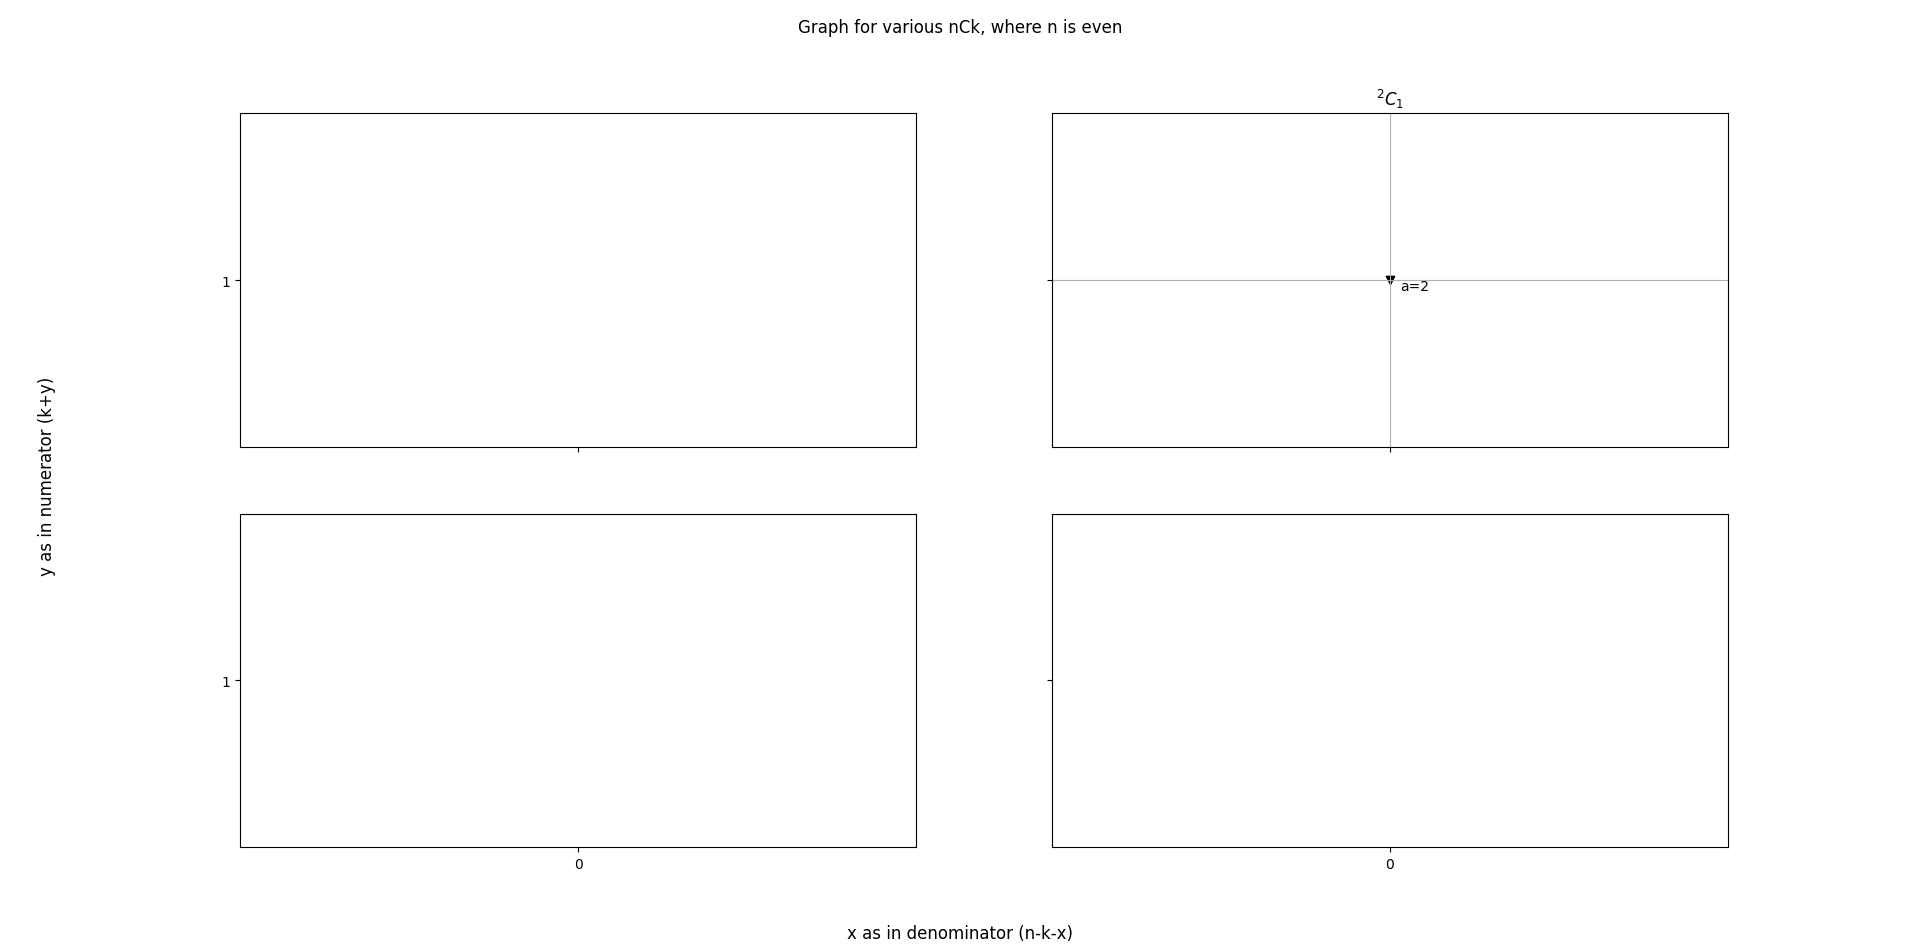
\includegraphics[width=\linewidth]{2Ck.png}
	\caption{Plot of $\Combination{2}{k}$}
	\label{2Ck}
\end{figure}
\begin{figure}[ph!]	
	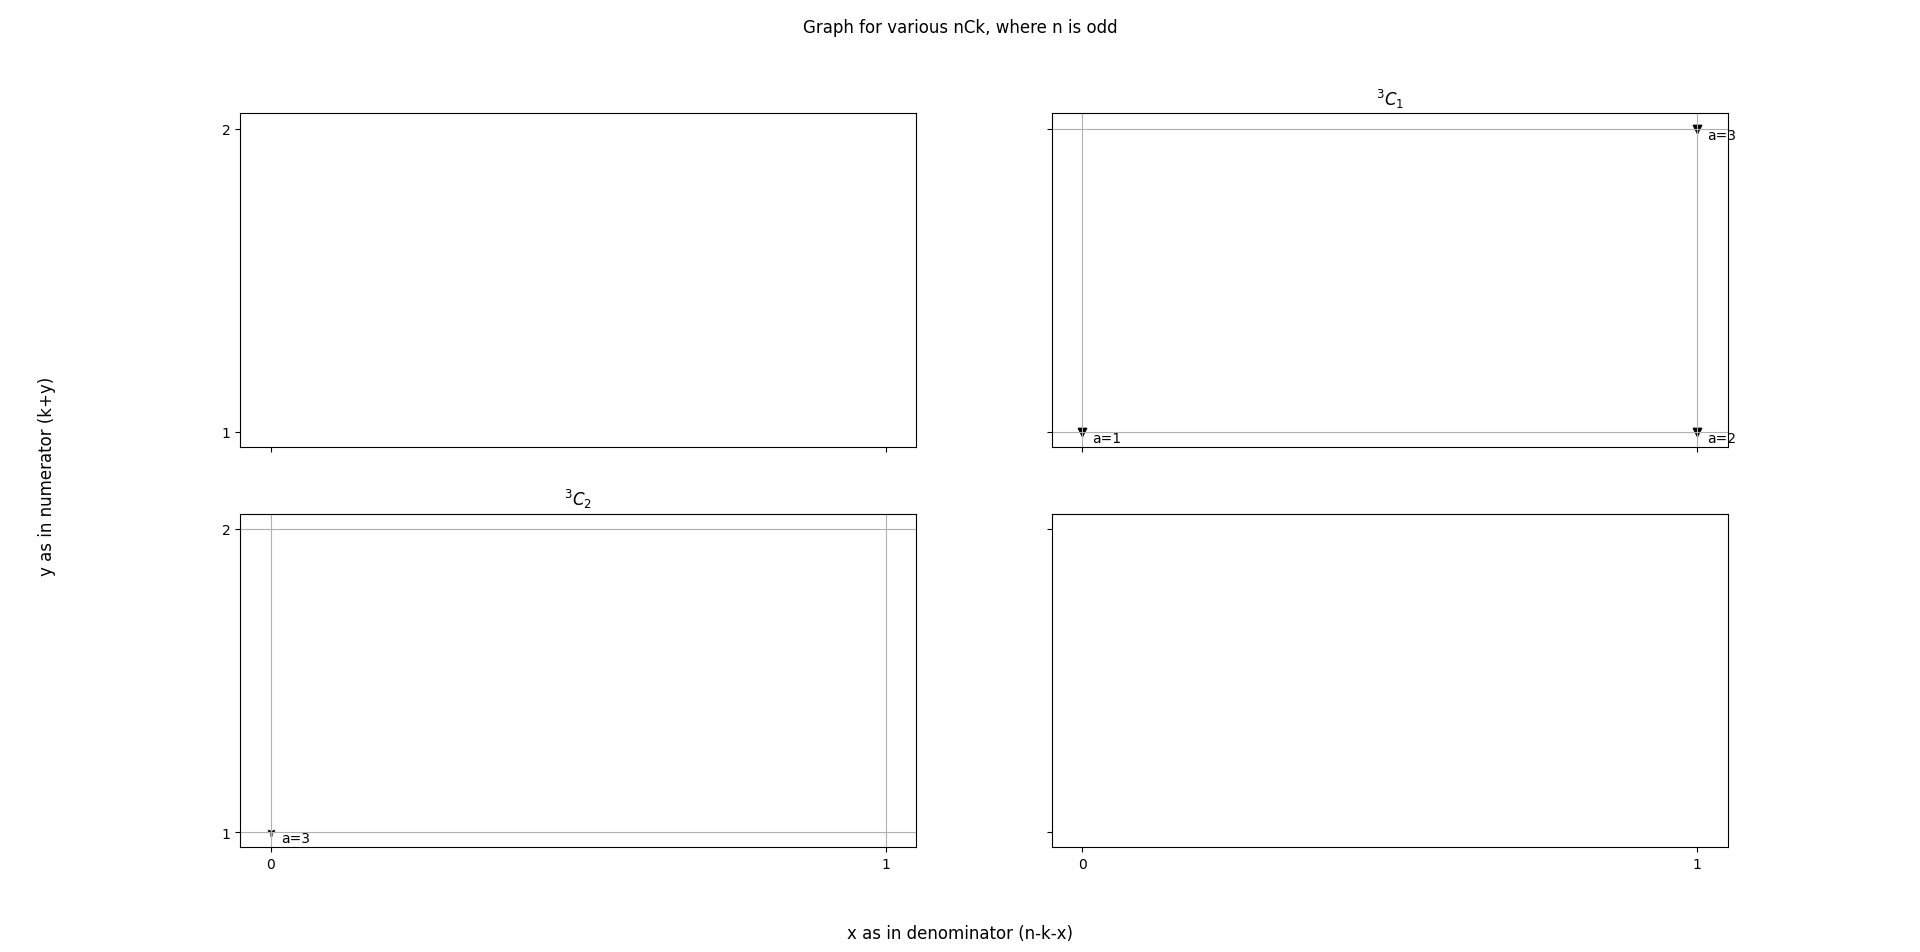
\includegraphics[width=\linewidth]{3Ck.png}
	\caption{Plot of $\Combination{3}{k}$}
	\label{3Ck}
\end{figure}
\begin{figure}[ph!]	
	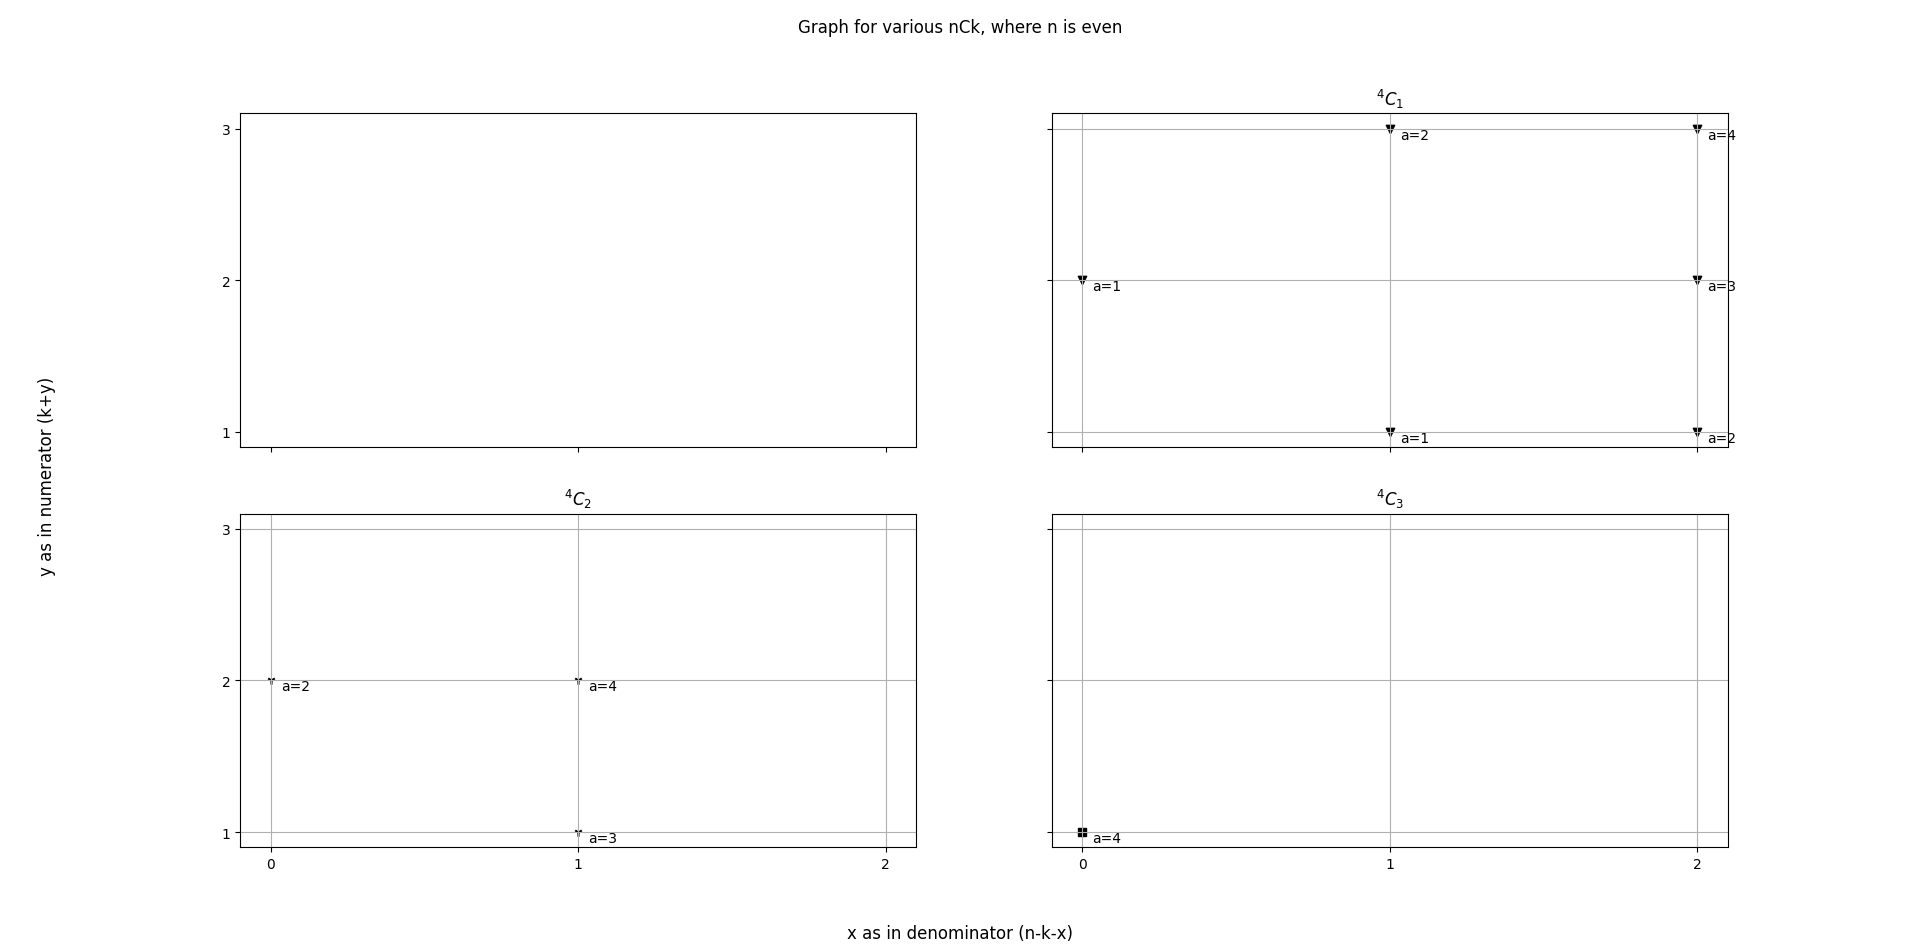
\includegraphics[width=\linewidth]{4Ck.png}
	\caption{Plot of $\Combination{4}{k}$}
	\label{4Ck}
\end{figure}
\begin{figure}[ph!]	
	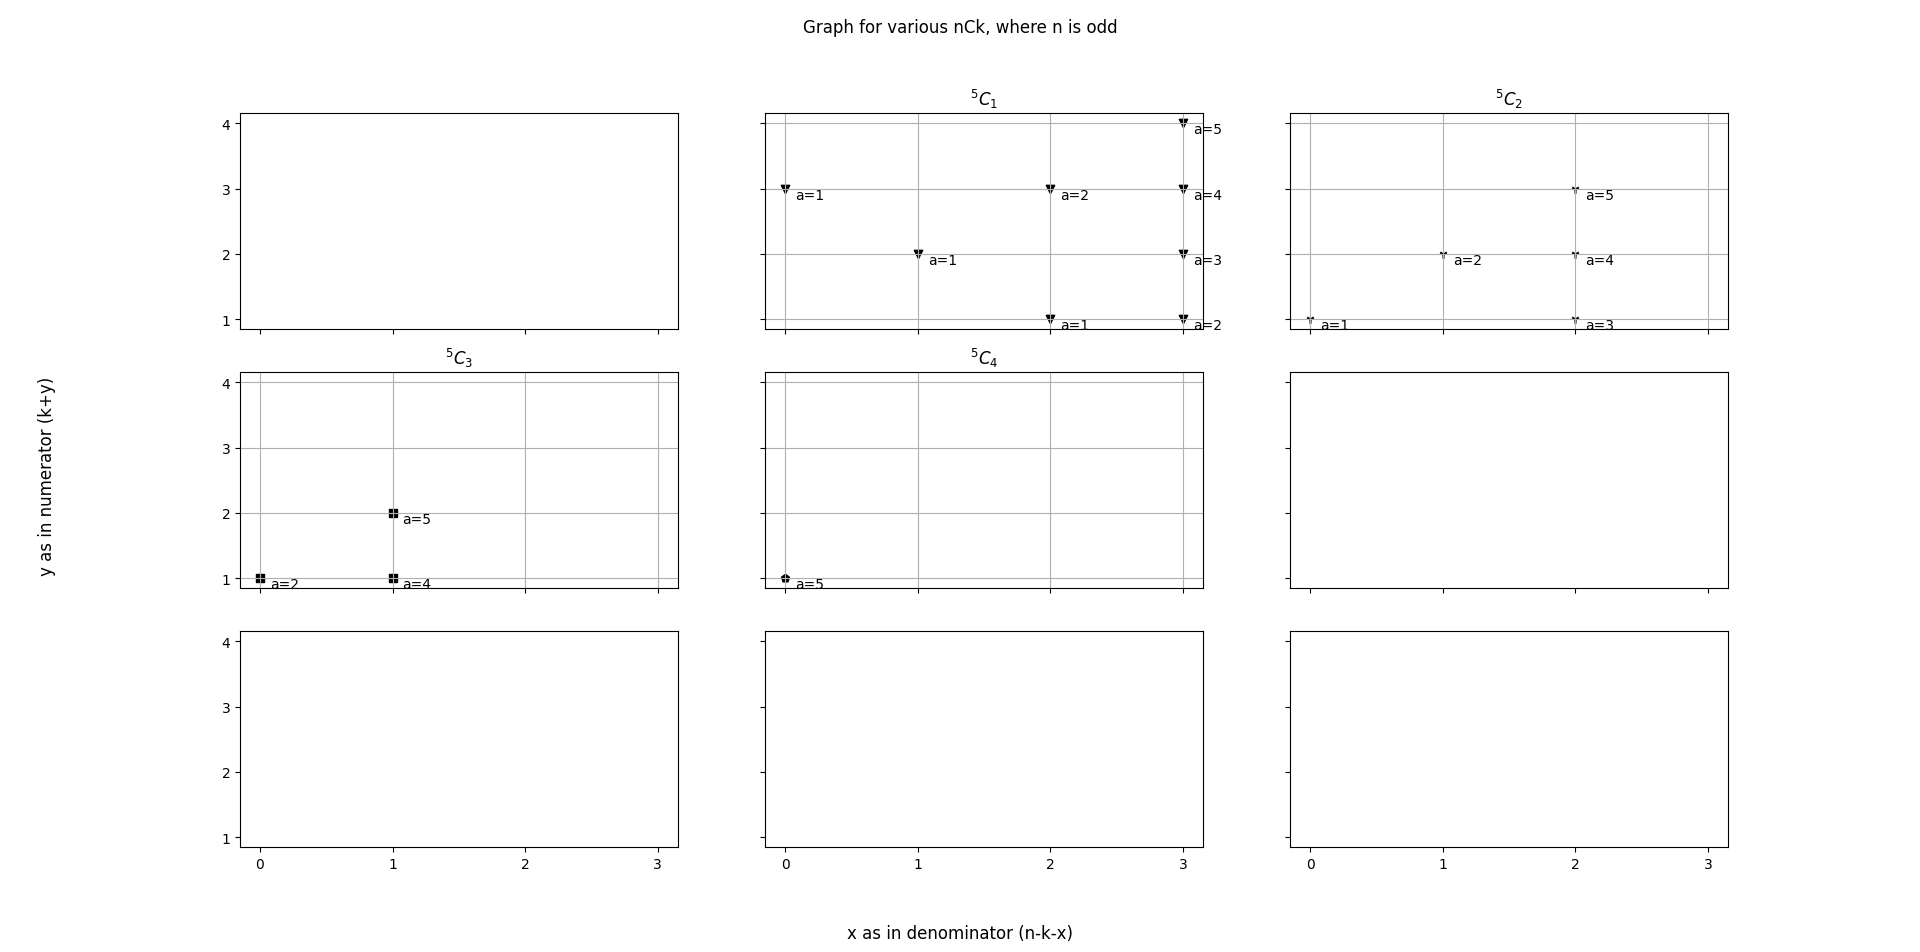
\includegraphics[width=\linewidth]{5Ck.png}
	\caption{Plot of $\Combination{5}{k}$}
	\label{5Ck}
\end{figure}
\begin{figure}[ph!]	
	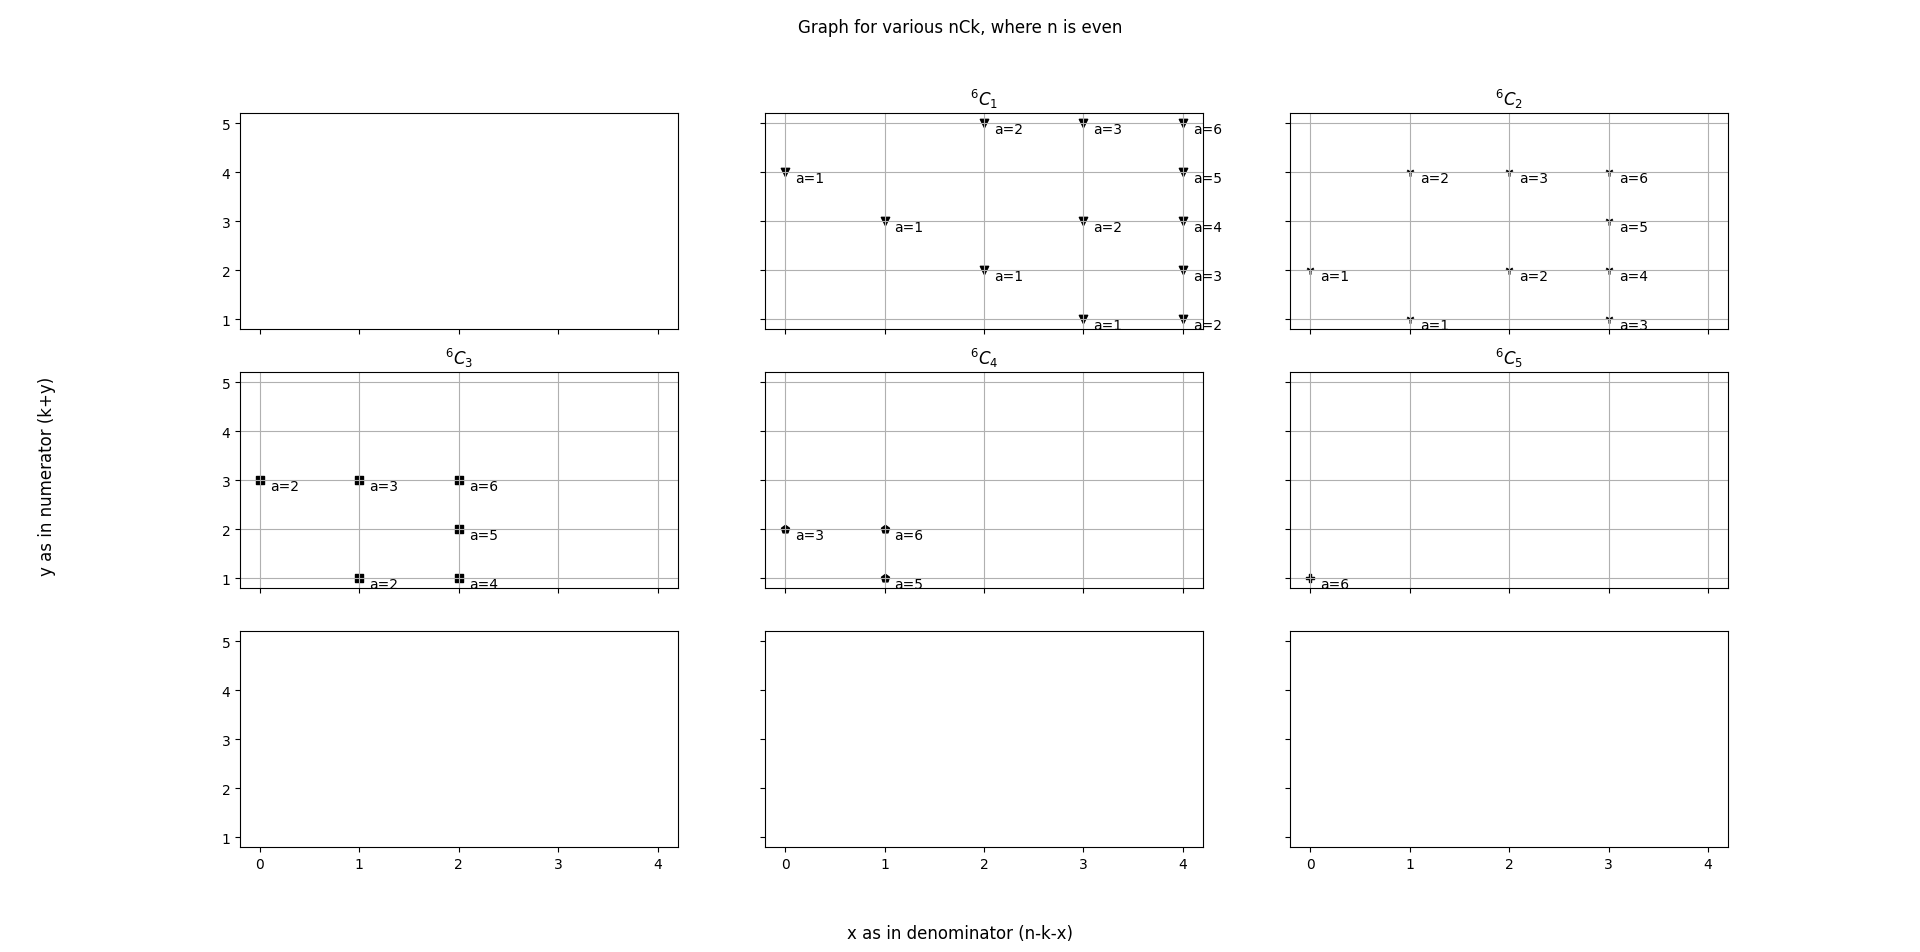
\includegraphics[width=\linewidth]{6Ck.png}
	\caption{Plot of $\Combination{6}{k}$}
	\label{6Ck}
\end{figure}
\begin{figure}[ph!]	
	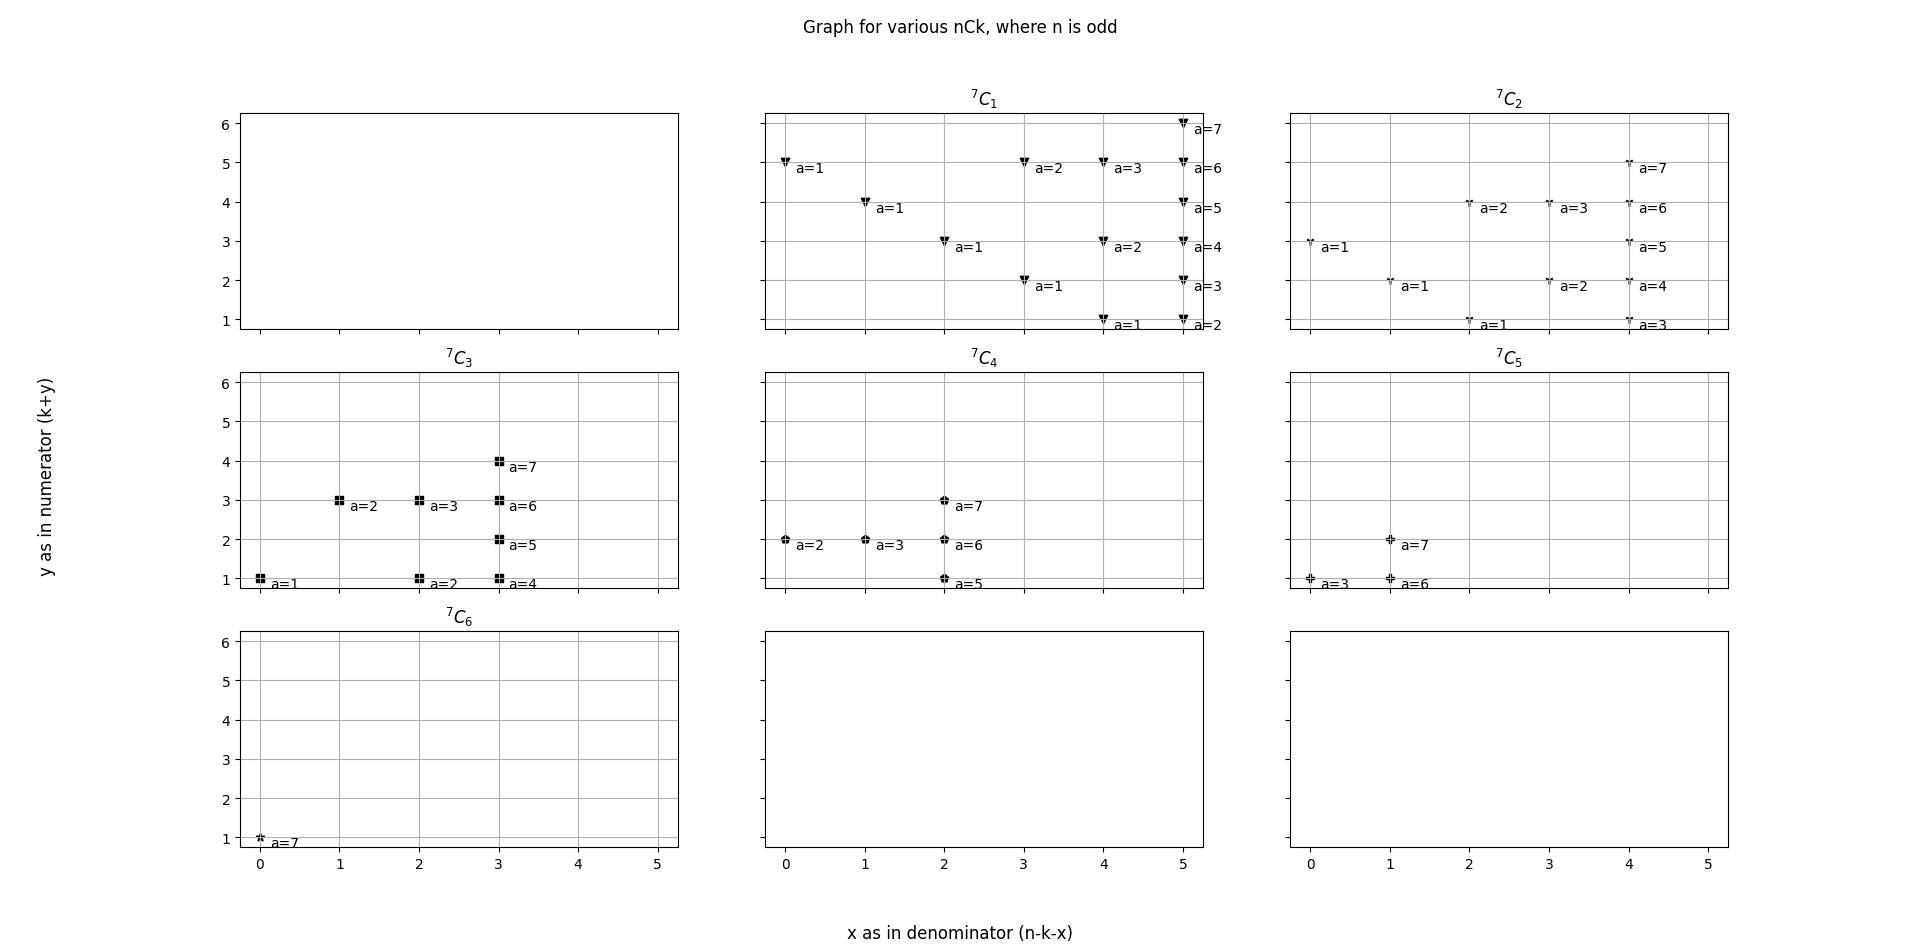
\includegraphics[width=\linewidth]{7Ck.png}
	\caption{Plot of $\Combination{7}{k}$}
	\label{7Ck}
\end{figure}
\begin{figure}[ph!]	
	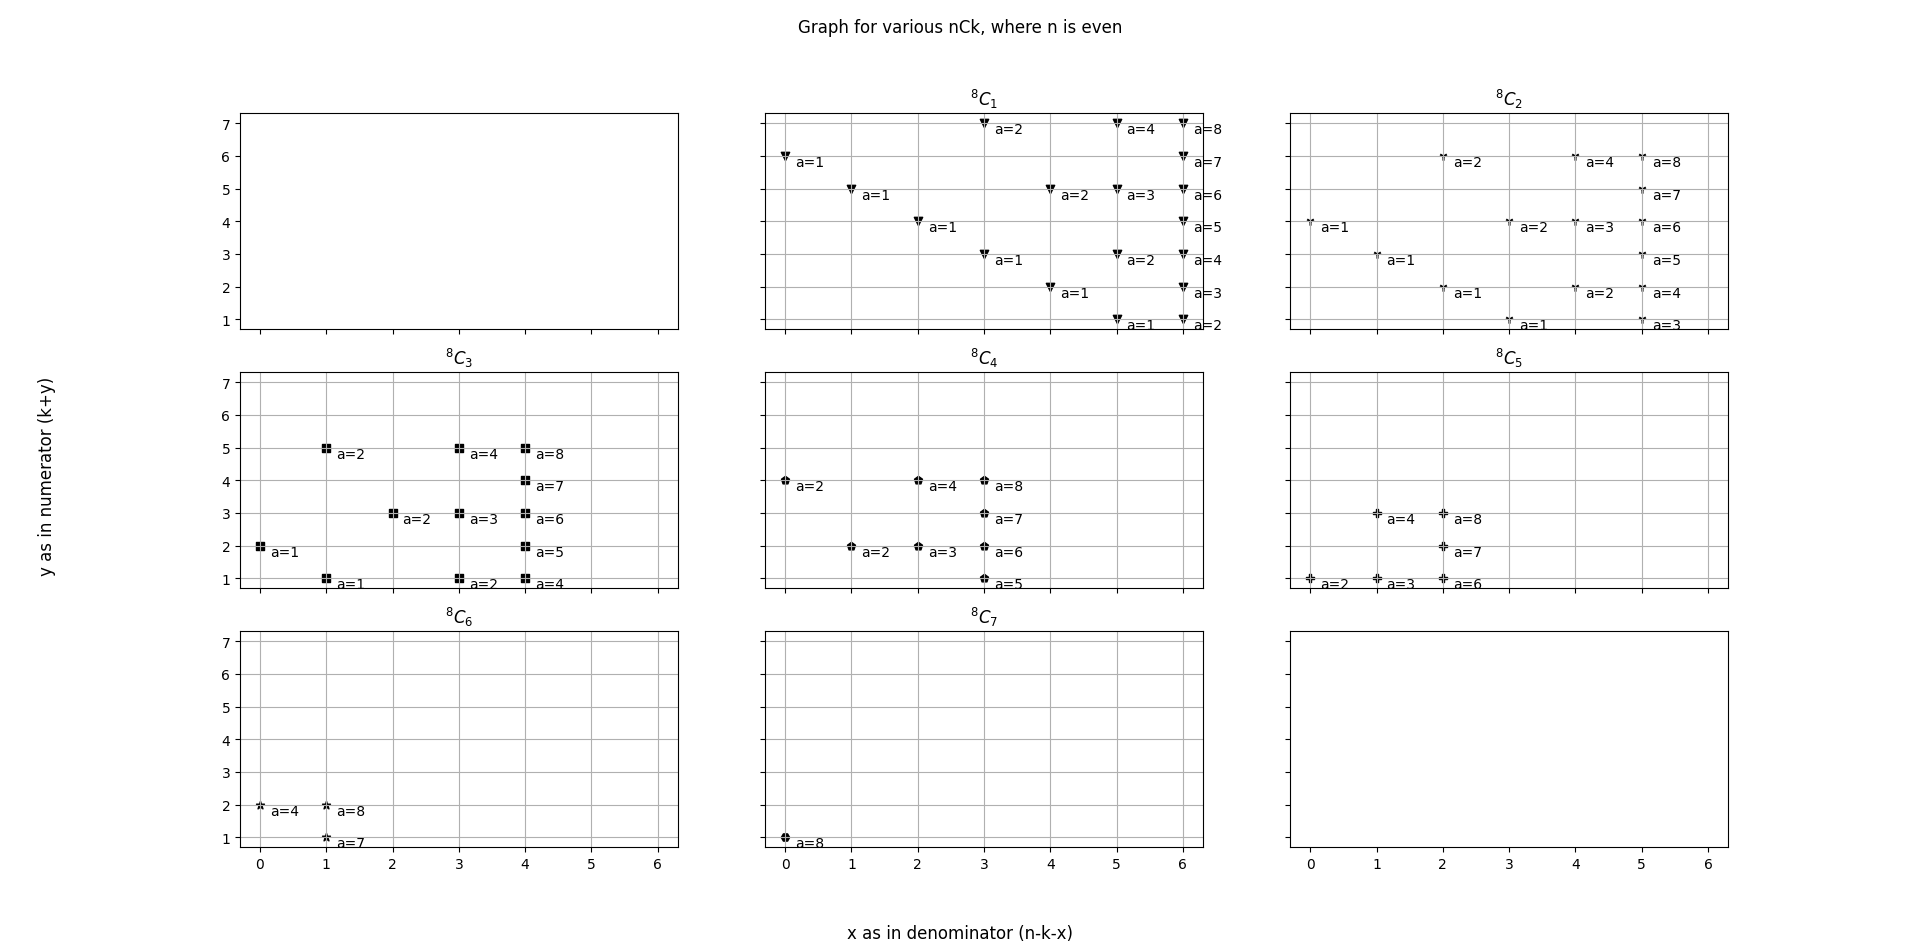
\includegraphics[width=\linewidth]{8Ck.png}
	\caption{Plot of $\Combination{8}{k}$}
	\label{8Ck}
\end{figure}
\begin{figure}[ph!]	
	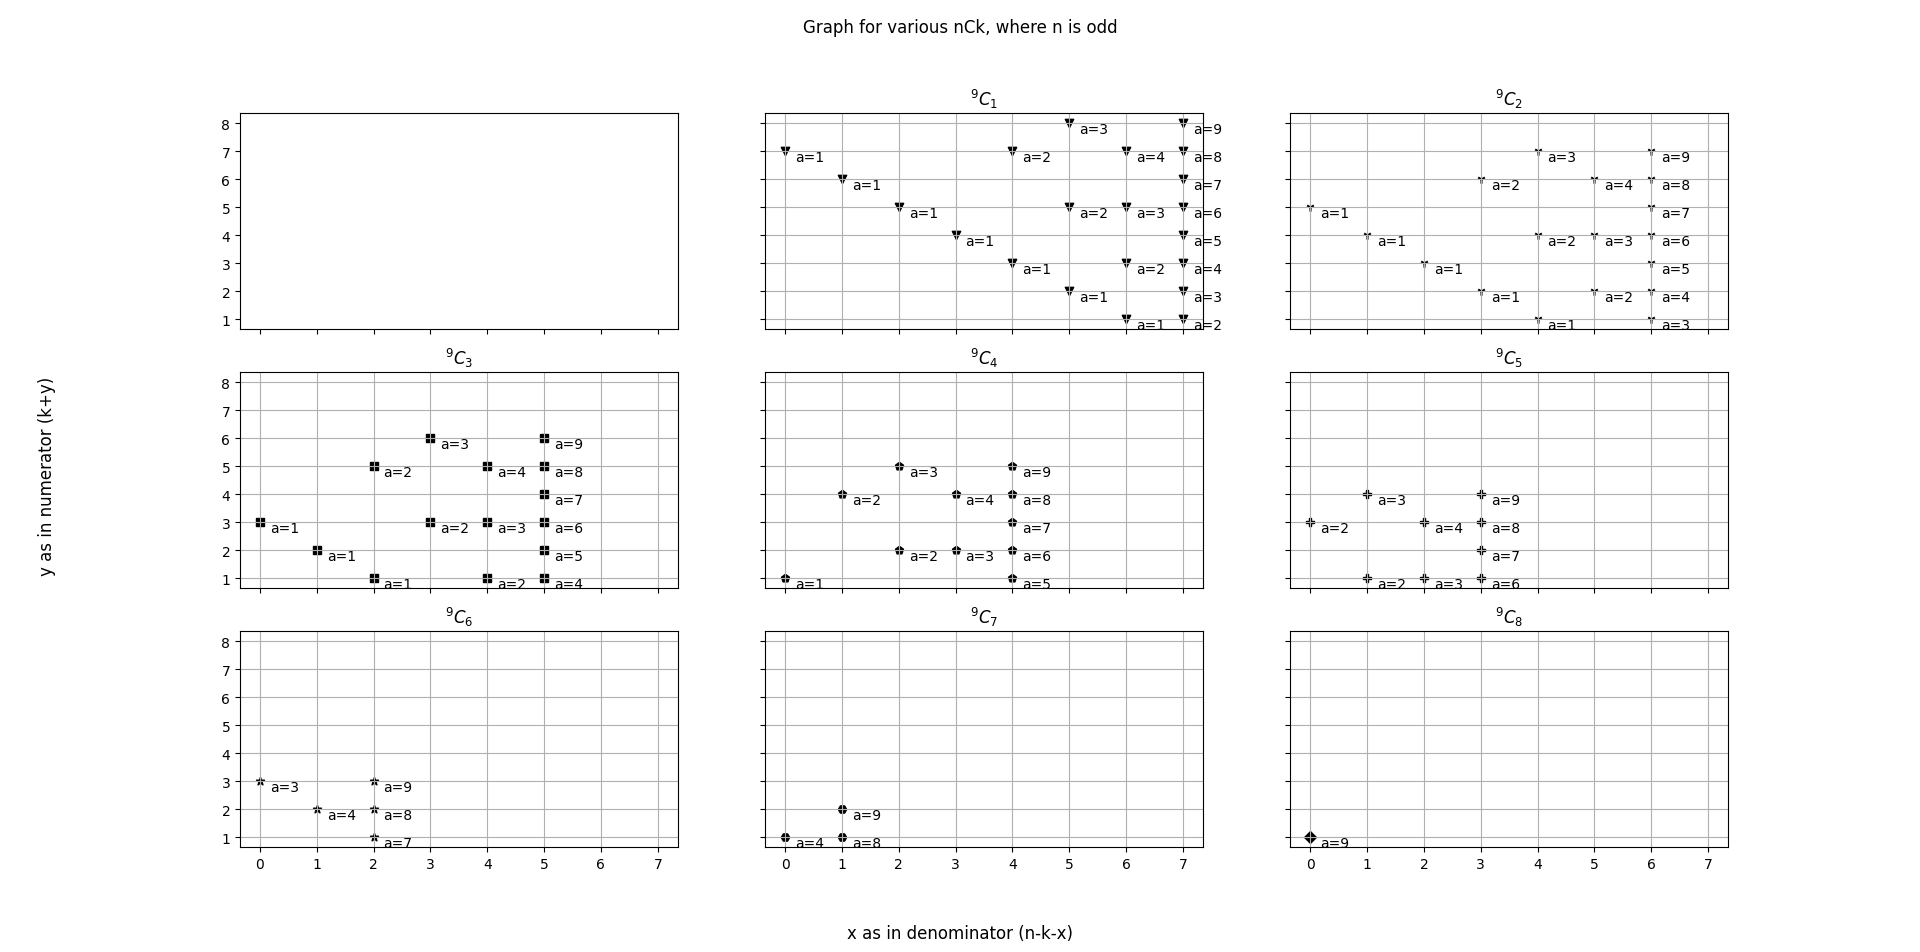
\includegraphics[width=\linewidth]{9Ck.png}
	\caption{Plot of $\Combination{9}{k}$}
	\label{9Ck}
\end{figure}
\begin{figure}[ph!]	
	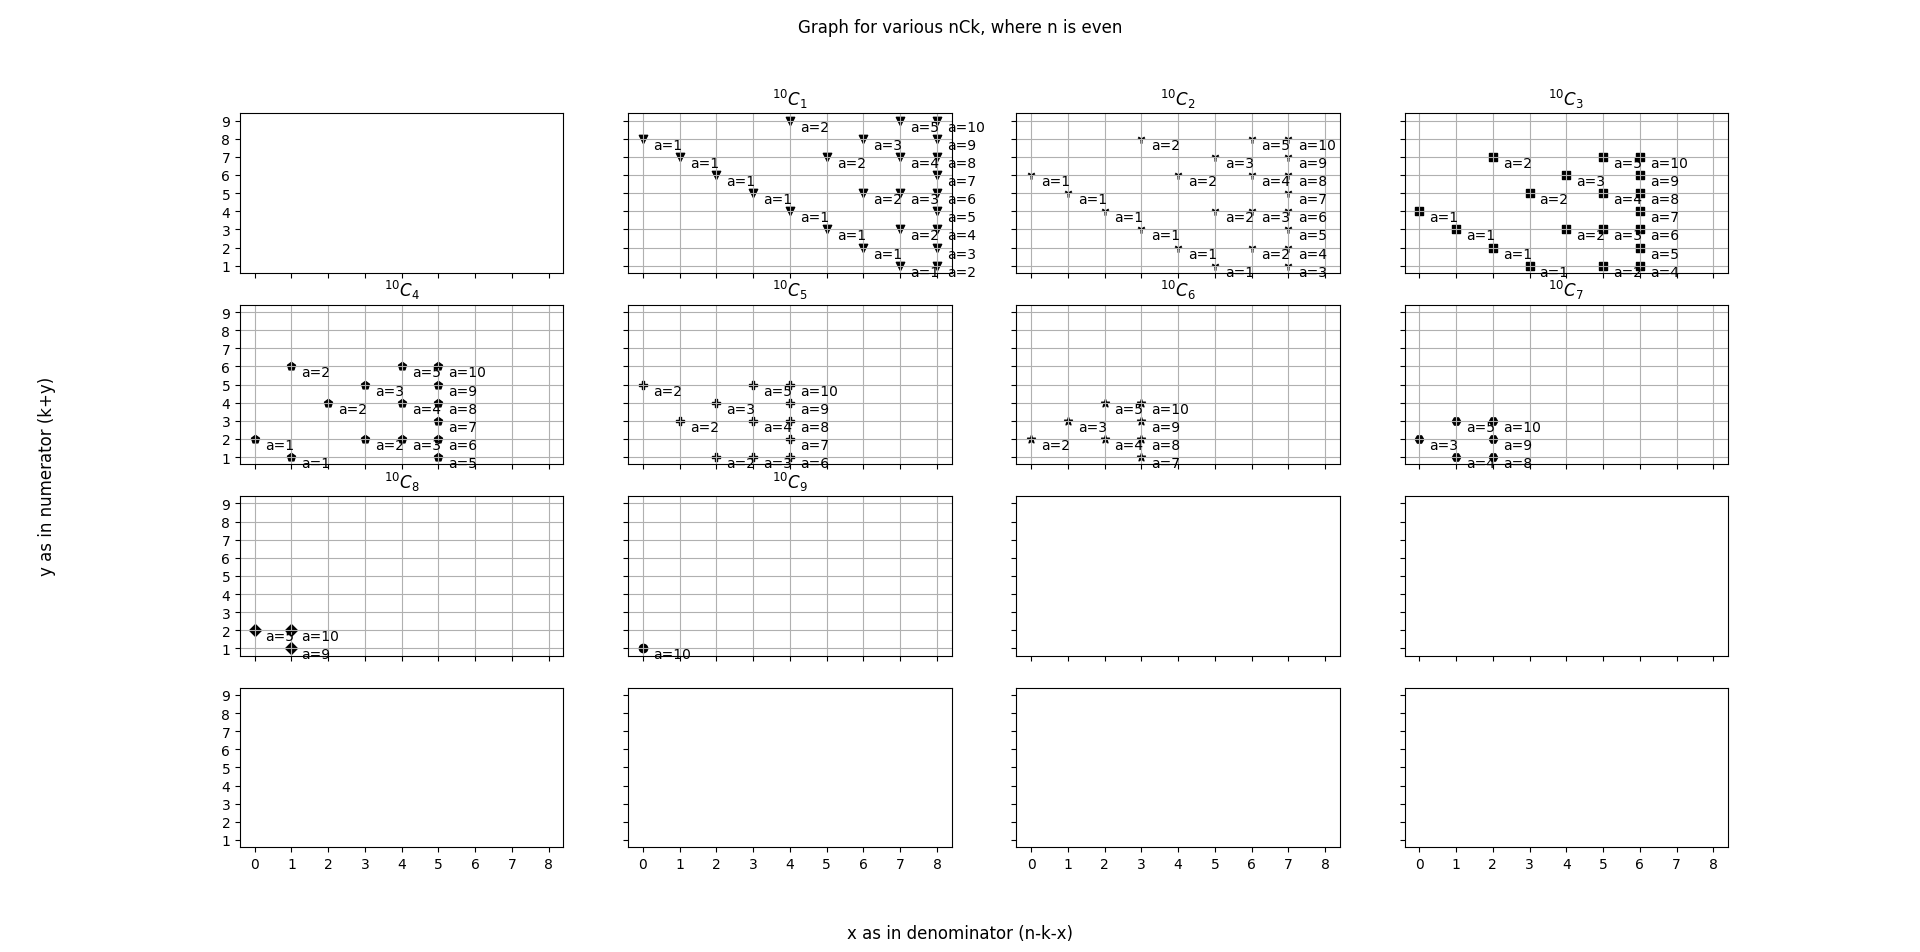
\includegraphics[width=\linewidth]{10Ck.png}
	\caption{Plot of $\Combination{10}{k}$}
	\label{10Ck}
\end{figure}	
\begin{figure}[ph!]	
	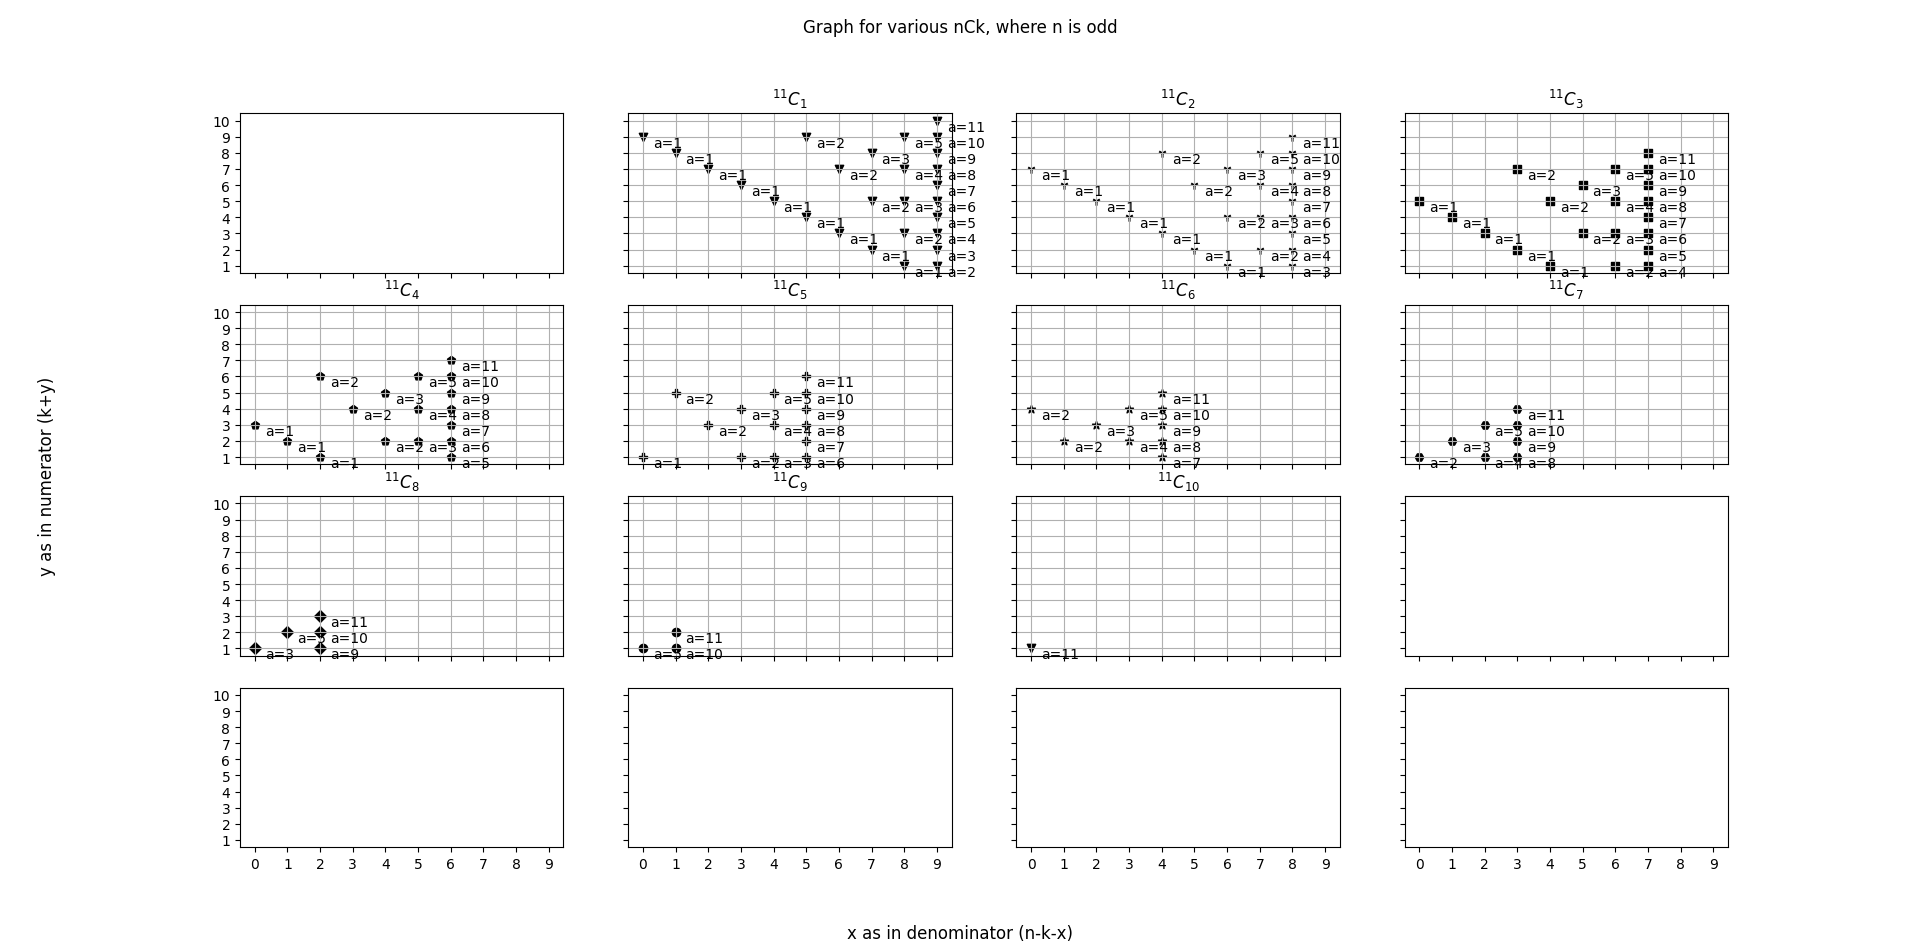
\includegraphics[width=\linewidth]{11Ck.png}
	\caption{Plot of $\Combination{11}{k}$}
	\label{11Ck}									
\end{figure}
\begin{figure}[ph!]	
	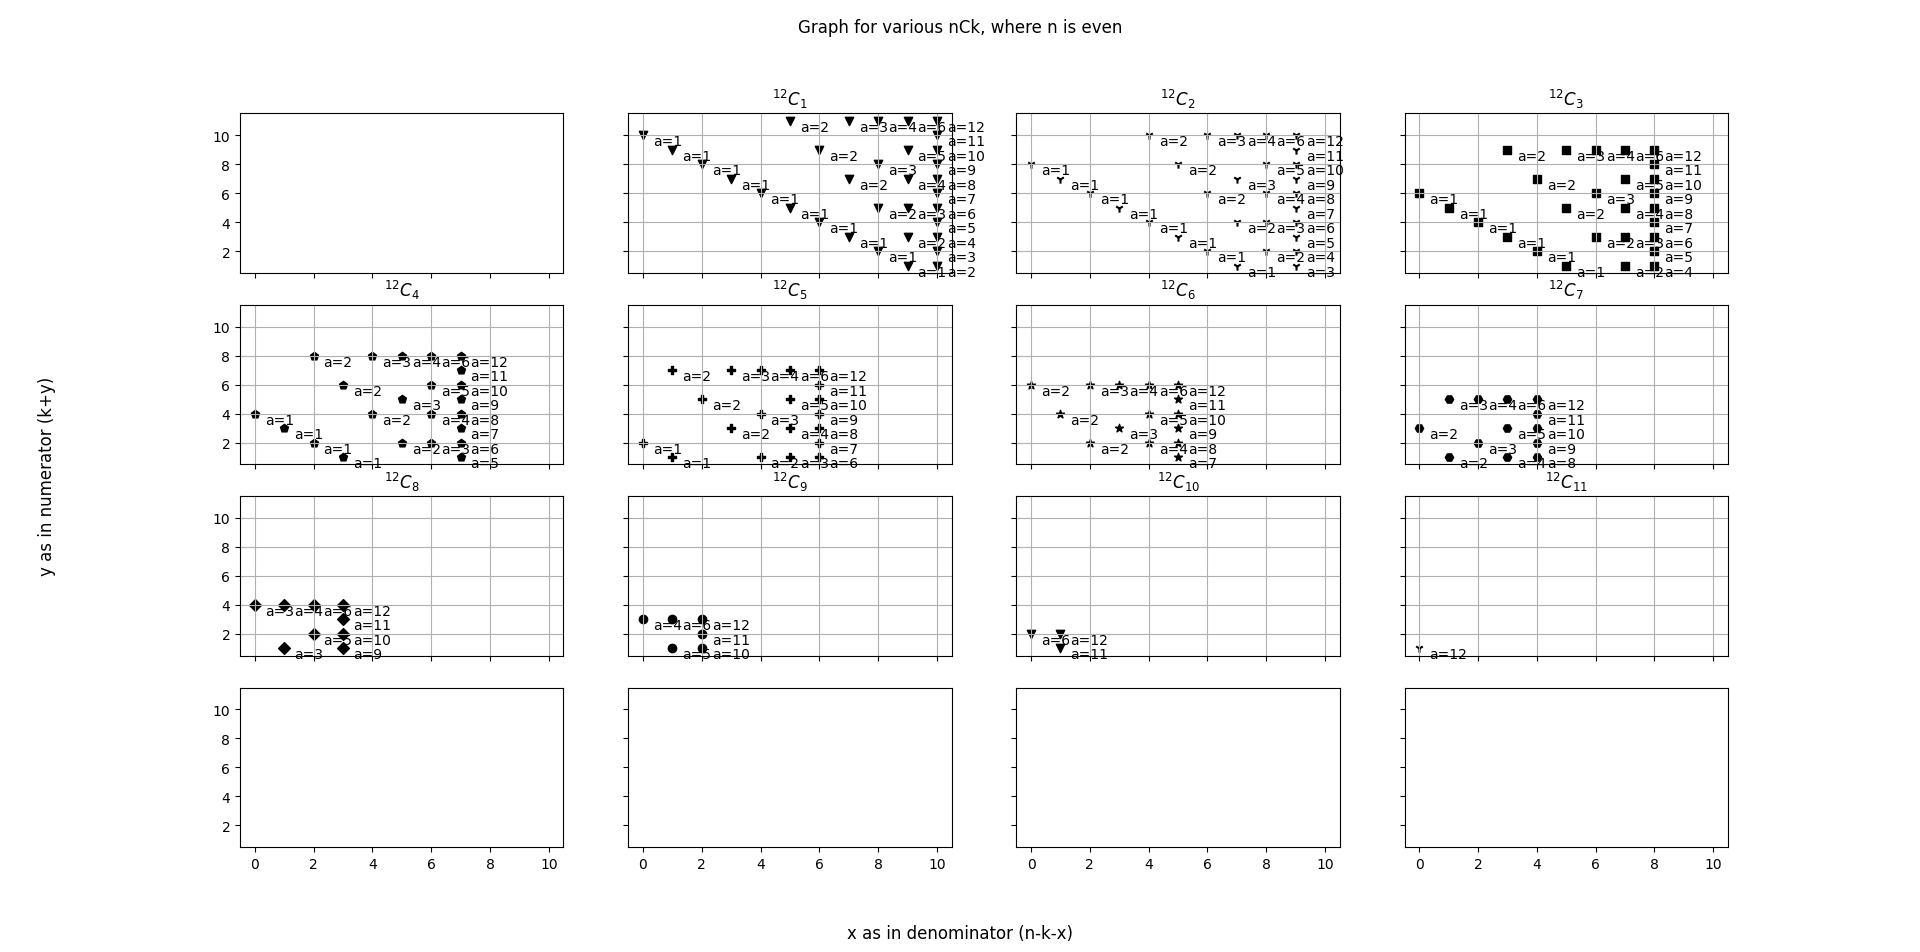
\includegraphics[width=\linewidth]{12Ck.png}
	\caption{Plot of $\Combination{12}{k}$}
	\label{12Ck}
\end{figure}	
\begin{figure}[ph!]	
	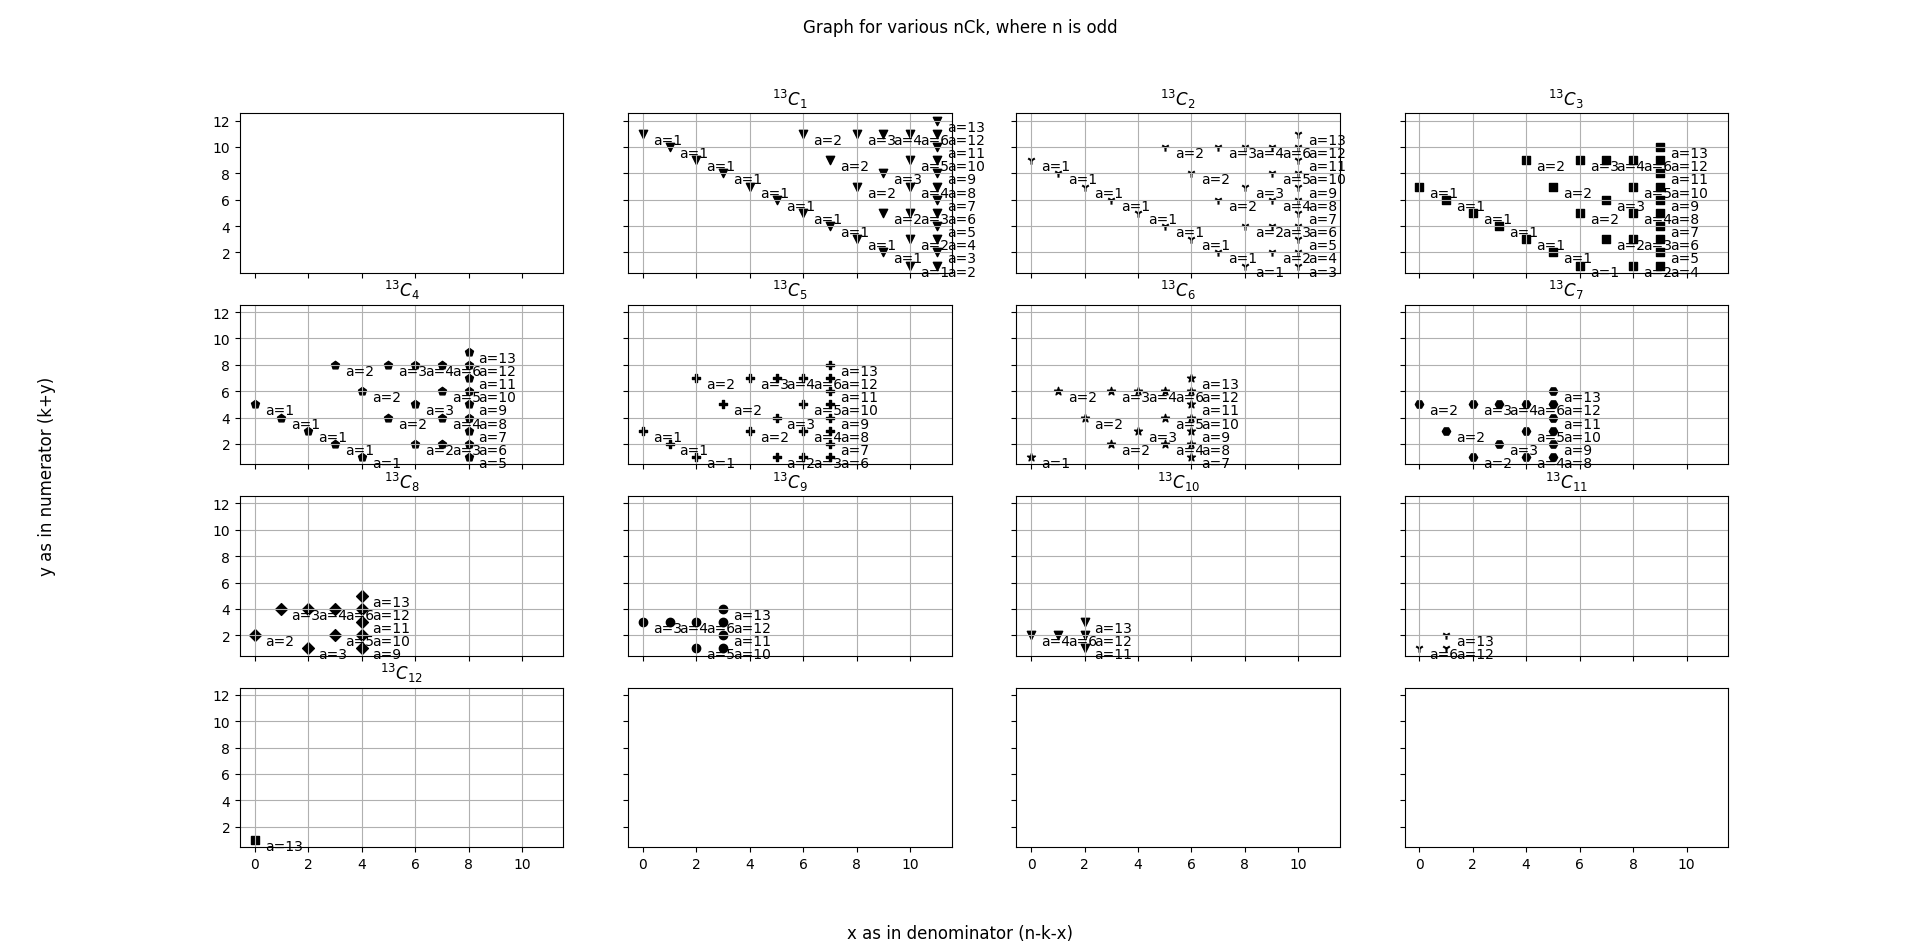
\includegraphics[width=\linewidth]{13Ck.png}
	\caption{Plot of $\Combination{13}{k}$}
	\label{13Ck}									
\end{figure}
\end{appendices}
\end{document}